\section{Problem formulation}
\label{sec:formulation}

\subsection{Configuration and assumptions}
\label{sec:config}
The configuration is two-dimensional (Figure~\ref{fig:geometry}). The fluid reference domain is
$\Om_f^0=\{-L_e\le X\le L+L_o,\;0\le Y\le H_0\}$: a rigid entrance section, a section of length $L$
facing the deformable wall, and a rigid exit section. The only deformable body is the solid strip
$\Om_s^0=[0,L]\times[H_0,H_0+d]$, of thickness $d$ and unit out-of-plane depth. Its lower face
$Y=H_0$ is the conjugate interface $\Ga_{\mathrm{if}}$; its upper face $Y=H_0+d$ is the outer face
$\Ga_h$, on which the thermal load is imposed. The strip ends $X=0$ and $X=L$ are pinned. Rigid,
adiabatic casing sections carry the strip at its ends, and the lower channel wall is rigid and
adiabatic. The geometry and the operating point are given in Table~\ref{tab:geometry}.

\begin{figure}[t]
\centering
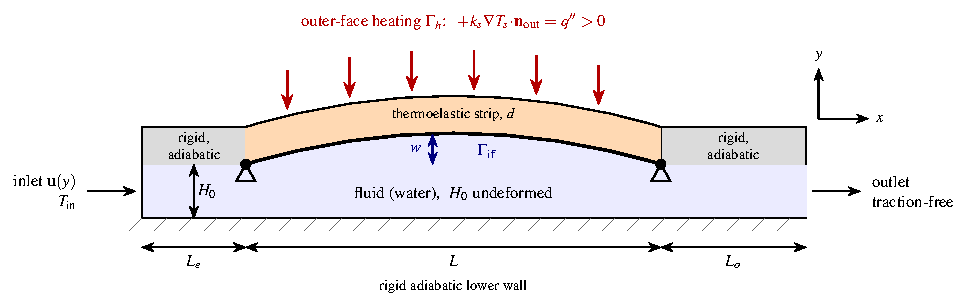
\includegraphics[width=\textwidth]{figures/fig1_geometry.pdf}
\caption{Configuration (schematic, not to scale; the strip thickness and the bow are exaggerated).
A thermoelastic strip of length $L$ and thickness $d$ forms part of the upper wall of a slit
channel of undeformed height $H_0$. The outer face $\Ga_h$ receives a prescribed heat flux $\qpp>0$
into the strip. With pinned ends the strip bows away from the channel: the interface deflection
$w$ is positive away from the channel and the passage widens.}
\label{fig:geometry}
\end{figure}

\begin{table}[t]
\centering\small
\caption{Geometry and operating point of the baseline (design values).}
\label{tab:geometry}
\begin{tabular}{@{}llll@{}}
\toprule
Quantity & Symbol & Value & Note \\
\midrule
Undeformed channel height & $H_0$ & \SI{0.50}{\milli\metre} & design input \\
Hydraulic diameter (slit) & $D_h=2H_0$ & \SI{1.0}{\milli\metre} & derived \\
Deformable (heated) length & $L$ & \SI{30}{\milli\metre} & design \\
Entrance / exit length & $L_e$, $L_o$ & \SI{10}{\milli\metre}, \SI{20}{\milli\metre} & design \\
Strip thickness & $d$ & \SI{3.0}{\milli\metre} & design \\
Mean inlet velocity & $U$ & \SI{0.050}{\metre\per\second} & design \\
Imposed outer-face heat flux & $\qpp$ & \SI{5.0}{\kilo\watt\per\square\metre} & design \\
\bottomrule
\end{tabular}
\end{table}

The following assumptions define the model; each is checked for the baseline in
Section~\ref{sec:baseline}.
\begin{description}[leftmargin=0pt,labelindent=0pt,style=unboxed,font=\normalfont\bfseries]
\item[A1] \emph{Plane strain.} The out-of-plane dimension is large compared with $H_0$ and $d$ and
the loading is uniform along it, so the fields are two-dimensional and $\varepsilon_{zz}=0$ in the
solid \citep{boley1960theory,timoshenko1970elasticity}.
\item[A2] \emph{Newtonian, constant-property water} at near-ambient temperature. Laminar, steady
flow ($\mathrm{Re}_{D_h}=\NumRe$); viscous dissipation and buoyancy are negligible at the baseline
(Section~\ref{sec:baseline}).
\item[A3] \emph{Homogeneous, isotropic, linearly thermoelastic solid} of constant $E$, $\nu$,
$\alpha$, $k_s$. The values are representative of an unfilled PEEK-class polymer
(Table~\ref{tab:props}); they are not frozen against a specific datasheet, and every derived number
scales with them.
\item[A4] \emph{Small strains and moderate rotations}, with the wall equation carried to the
von K\'arm\'an beam--column level of Section~\ref{sec:beamcolumn}.
\item[A5] \emph{Steady flow and energy, quasi-static solid.} The structural wave-crossing time of the
strip, $d\sqrt{\rho_s/E}\approx\SI{1.8}{\micro\second}$, is many orders of magnitude shorter than the
transport times, so inertia is omitted.
\item[A6] \emph{Perfect thermal contact} at $\Ga_{\mathrm{if}}$: temperature and normal heat flux are
continuous; no contact resistance.
\item[A7] \emph{Ideal pinned ends.} At $X=0,L$ the vertical displacement vanishes, the mean axial
displacement over the end edge vanishes, the applied moment is zero, and the heat flux is zero. This
is a pin and not a clamp: a clamp forbids end rotation, and a clamped strip at uniform curvature
does not bow at all (Section~\ref{sec:freecurv}).
\item[A8] \emph{Idealised heater.} The heater is represented only by a uniform flux $\qpp$ entering
the solid through $\Ga_h$. Heater construction, heater--wall contact resistance and heat loss from
the outer face are not modelled; all of $\qpp$ is assumed to enter the strip.
\item[A9] \emph{Rigid casing as a support, not as a contact.} The casing fixes the end conditions and
the reference pressure of the cavity above the strip (equal to the outlet datum). The model contains
no contact between the deformed strip and the casing and no casing clearance; the cavity above the
strip is assumed to leave room for the computed deflection.
\end{description}

\subsection{Governing equations}
\label{sec:governing}
\emph{Fluid.} On the deformed fluid domain $\Om_f$ (Section~\ref{sec:ale}), steady incompressible
flow with constant properties obeys, in the standard form \citep{bird1960transport},
\begin{align}
\nabla\!\cdot\bu&=0, \label{eq:cont}\\
\rho\,(\bu\!\cdot\!\nabla)\bu&=-\nabla p+\mu\nabla^2\bu, \label{eq:mom}\\
\rho c_p\,(\bu\!\cdot\!\nabla)T_f&=k_f\nabla^2T_f. \label{eq:fe}
\end{align}
\emph{Solid.} On the reference configuration $\Om_s^0$ steady conduction \citep{carslaw1947conduction}
and linear thermoelastic equilibrium without inertia hold,
\begin{align}
\nabla\!\cdot(k_s\nabla T_s)&=0, \label{eq:cond}\\
\nabla\!\cdot\bsig=\bm 0,\qquad
\bsig&=2\mu_L\beps+\lambda(\operatorname{tr}\beps)\bI-\beta\theta\bI,\qquad
\beps=\tfrac12\!\left(\nabla\bd+\nabla\bd^{\mathsf T}\right), \label{eq:solid}
\end{align}
with $\theta=T_s-T_{\mathrm{ref}}$, Lam\'e parameters $\lambda,\mu_L$ and thermoelastic pressure
coefficient $\beta=E\alpha/(1-2\nu)$ \citep{boley1960theory}. In plane strain the out-of-plane
stress is $\sigma_{zz}=\nu(\sigma_{xx}+\sigma_{yy})-E\alpha\theta$ and is part of the stress state; all
stresses reported below are total Cauchy stresses. The deformation-heating source of the transient
thermoelastic energy equation vanishes identically in a steady state, so \eqref{eq:cond} is exact
for the steady problem.

\emph{Reduced wall equation.} For design estimates the strip is treated as an Euler--Bernoulli strip
of flexural rigidity per unit depth $D_s=Ed^3/[12(1-\nu^2)]$, the wide-strip value appropriate to plane strain,
\begin{equation}
D_s\,w^{\prime\prime\prime\prime}=p(x),\qquad w(0)=w(L)=w^{\prime\prime}(0)=w^{\prime\prime}(L)=0,
\label{eq:beam}
\end{equation}
where $p$ is the fluid pressure acting on the strip (positive pushes the strip away from the channel).
This equation is used for estimates and benchmarks only; the two-dimensional system
\eqref{eq:cond}--\eqref{eq:solid} is the model.

\subsection{Deformed domain}
\label{sec:ale}
The fluid problem is posed on the domain occupied by the fluid in the converged steady state. Given
the solid displacement on $\Ga_{\mathrm{if}}^0$, a mesh displacement $\bwhat$ is obtained on
$\Om_f^0$ from a pseudo-elastic extension problem with $\bwhat=\bd$ on $\Ga_{\mathrm{if}}^0$ and
$\bwhat=\bm 0$ on rigid boundaries, and $\Om_f=\{X+\bwhat(X)\}$. No time derivative appears, so no mesh
velocity or geometric-conservation-law constraint arises in the steady problem
\citep{lesoinne1996geometric}.

\subsection{Sign conventions, interface and boundary conditions}
\label{sec:bc}
A single unit normal $\bn$, pointing from the fluid into the solid, is used on $\Ga_{\mathrm{if}}$.
Pressure is positive in compression and stress is positive in tension. The coordinate $y$ points from
the fluid into the solid. The deflection $w$ is measured \emph{away from the channel},
$w=+d_2$ with $d_2$ the displacement in $+y$; the thermal curvature $\kth>0$ is the curvature that
bows the strip away from the channel, and within small slopes $\kappa=-w^{\prime\prime}$. The heat flux
vector is $\bm q=-k\nabla T$, and $\qpp>0$ denotes heat \emph{supplied} to the solid.

On the deformed interface the subsystems exchange kinematics, traction and heat:
\begin{align}
\bu&=\bm 0 && \text{(no slip, steady form of }\bu=\partial_t\bd), \label{eq:ifkin}\\
\bsig\bn&=\left(-p\bI+2\mu\bD(\bu)\right)\bn && \text{(traction continuity)}, \label{eq:iftrac}\\
T_f&=T_s && \text{(temperature continuity)}, \label{eq:iftemp}\\
-k_f\nabla T_f\!\cdot\!\bn&=-k_s\nabla T_s\!\cdot\!\bn && \text{(normal heat-flux continuity)}, \label{eq:ifflux}
\end{align}
with $\bD(\bu)=\tfrac12(\nabla\bu+\nabla\bu^{\mathsf T})$. The exterior conditions are listed in
Table~\ref{tab:bcs}. Condition B5 makes the sign of the thermal load explicit: with the outward
normal $\bn_{\mathrm{out}}=+\bm e_y$ of the solid on $\Ga_h$, the flux $\bm q\cdot\bn_{\mathrm{out}}=-k_s\partial_yT_s$
equals $-\qpp$ (inward), so $k_s\,\partial_yT_s=+\qpp>0$: the temperature rises towards the outer
face, which is therefore the hot face.

\begin{table}[t]
\centering\small
\caption{Boundary conditions. $\bn_{\mathrm{out}}$ is the outward normal of the solid.}
\label{tab:bcs}
\begin{tabular}{@{}p{0.7cm}p{3.2cm}p{9.2cm}@{}}
\toprule
ID & Boundary & Condition \\
\midrule
B1 & inlet $x=-L_e$ & $\bu=6U\frac{y}{H_0}\left(1-\frac{y}{H_0}\right)\bm e_x$, $T_f=T_{\mathrm{in}}$ \\
B2 & outlet $x=L+L_o$ & traction-free (do-nothing) outflow, $\partial_nT_f=0$ \\
B3 & lower wall $y=0$ & $\bu=\bm 0$, $\partial_nT_f=0$ (rigid, adiabatic) \\
B4 & rigid casing sections & $\bu=\bm 0$, $\partial_nT_f=0$ \\
B5 & outer face $\Ga_h^0$ & $+k_s\nabla T_s\!\cdot\!\bn_{\mathrm{out}}=\qpp$ with $\qpp>0$ heat supplied to the solid \\
B6 & strip ends $X=0,L$ & $d_2=0$, $\langle d_1\rangle=0$ (edge mean), zero applied moment, $\partial_nT_s=0$ \\
B7 & remaining solid faces & zero traction, zero heat flux \\
B8 & interface $\Ga_{\mathrm{if}}$ & \eqref{eq:ifkin}--\eqref{eq:ifflux} \\
\bottomrule
\end{tabular}
\end{table}

\subsection{Material data}
\label{sec:props}
Table~\ref{tab:props} lists the properties. Water values are standard near-ambient data. The solid
values are representative of unfilled PEEK and are datasheet-representative, not grade-specific.

\begin{table}[t]
\centering\small
\caption{Material properties used in all calculations.}
\label{tab:props}
\begin{tabular}{@{}llll@{}}
\toprule
Property & Symbol & Value & Unit \\
\midrule
Water density, viscosity & $\rho$, $\mu$ & $1.0\times10^{3}$, $1.0\times10^{-3}$ & \si{\kilo\gram\per\cubic\metre}, \si{\pascal\second} \\
Water specific heat, conductivity & $c_p$, $k_f$ & $4.18\times10^{3}$, $0.60$ & \si{\joule\per\kilo\gram\per\kelvin}, \si{\watt\per\metre\per\kelvin} \\
Solid Young's modulus, Poisson ratio & $E$, $\nu$ & $3.6\times10^{9}$, $0.40$ & \si{\pascal}, -- \\
Solid expansion coefficient & $\alpha$ & $5.0\times10^{-5}$ & \si{\per\kelvin} \\
Solid conductivity & $k_s$ & $0.25$ & \si{\watt\per\metre\per\kelvin} \\
Solid yield stress (guard only) & $\sigma_y$ & $9\times10^{7}$ & \si{\pascal} \\
\bottomrule
\end{tabular}
\end{table}
